% Extracted from LaTeX-examples-master/tikz/triangle-9-point-circle.
% This focused fixture retains the original triangle and midpoint construction.
\documentclass[border=3pt]{standalone}
\usepackage{tikz}
\usepackage{tkz-euclide}

\begin{document}
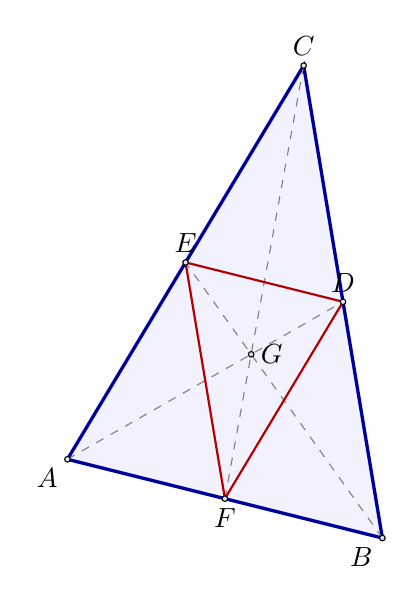
\begin{tikzpicture}
  \tkzDefPoints{0/1/A,4/0/B,3/6/C}
  \tkzDefMidPoint(A,B)\tkzGetPoint{F}
  \tkzDefMidPoint(A,C)\tkzGetPoint{E}
  \tkzDefMidPoint(B,C)\tkzGetPoint{D}
  \tkzInterLL(A,D)(B,E)\tkzGetPoint{G}

  \fill[blue!5] (A) -- (B) -- (C) -- cycle;
  \draw[very thick,blue!60!black] (A) -- (B) -- (C) -- cycle;
  \draw[dashed,gray] (A) -- (D) (B) -- (E) (C) -- (F);
  \draw[red!70!black,thick] (F) -- (D) -- (E) -- cycle;

  \tkzDrawPoints(A,B,C,D,E,F,G)
  \tkzLabelPoints[below left](A,B)
  \tkzLabelPoints[above](C,D,E)
  \tkzLabelPoints[below](F)
  \tkzLabelPoints[right](G)
\end{tikzpicture}
\end{document}
